\newcommand{\erfc}{\mathrm{erfc}}
\newcommand{\erf}{\mathrm{erf}}
\chapter{Решение диффузионной задачи на полупрямой методом
синус-преобразования. Интерпретация решения.}

Эта задача имеет следующий вид:
\[
    \left\{ \begin{array}{rl}
        \text{ДУЧП:} & \ds \pder{u}{t} = \alpha^2\ppder{u}{x}; x \in (0, \infty)
        \vspace*{.4em} \\
        \text{ГУ:} & u(0, t) = A; \\
        \text{НУ:} & u(x, 0) = 0.
    \end{array} \right.
\]

Выполним синус-преобразование по переменной \( x \):
\begin{align*}
    & u \to \bar{u}; \\
    & \ppder{u}{x} \to \frac{2}{\pi}\omega u(0, t) - \omega^2\bar{u}.
\end{align*}

Тогда исходная задача преобразуется к следующей задаче Коши:
\begin{align*}
    & \der{\bar{u}}{t}+\alpha^2\omega^2\bar{u} = \frac{2}{pi}A\omega\alpha^2; \\
    & \bar{u}(0) = 0.
\end{align*}

Решая её, получаем:
\( \ds
    \bar{u}(t) = \frac{2A}{\pi\omega}\Bigl(1-\e^{-\alpha^2\omega^2 t}\Bigr)
\).

Выполнив обратное синус-преобразование, получим:
\( \ds
    u(x, t) = A\cdot\erfc\left(\frac{x}{2\alpha\sqrt{t}}\right)
\),

где
\( \ds
    \erfc(x) = \sqrt\frac{2}{\pi} \int\limits_x^{+\infty} \e^{-t^2}\d t
\) -- функция, дополнительная к интегралу вероятности.

\begin{figure}[h!]
    \center
    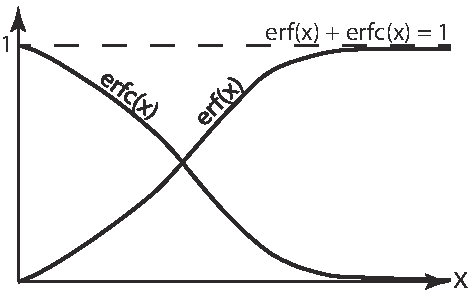
\includegraphics[width=.56\textwidth]{11_erfc} \hfill
    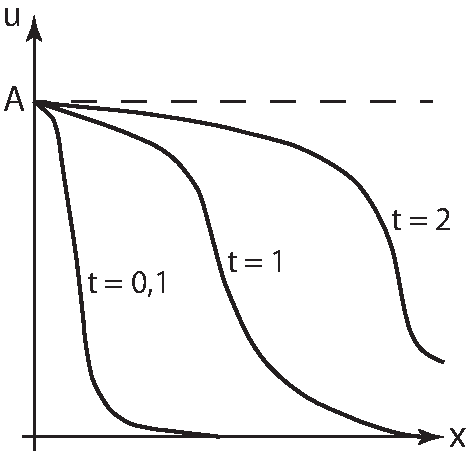
\includegraphics[width=.37\textwidth]{11_u(x)} \\
    \parbox{.56\textwidth}{\centering Вид функций \( \erfc(x) \) и \( \erf(x) \)}
    \hfill
    \parbox{.37\textwidth}{\centering Вид решения в различные моменты времени}
\end{figure}
\newpage
